\documentclass{standalone}
\usepackage{pgfplots}
\pgfplotsset{compat=newest}

\begin{document}
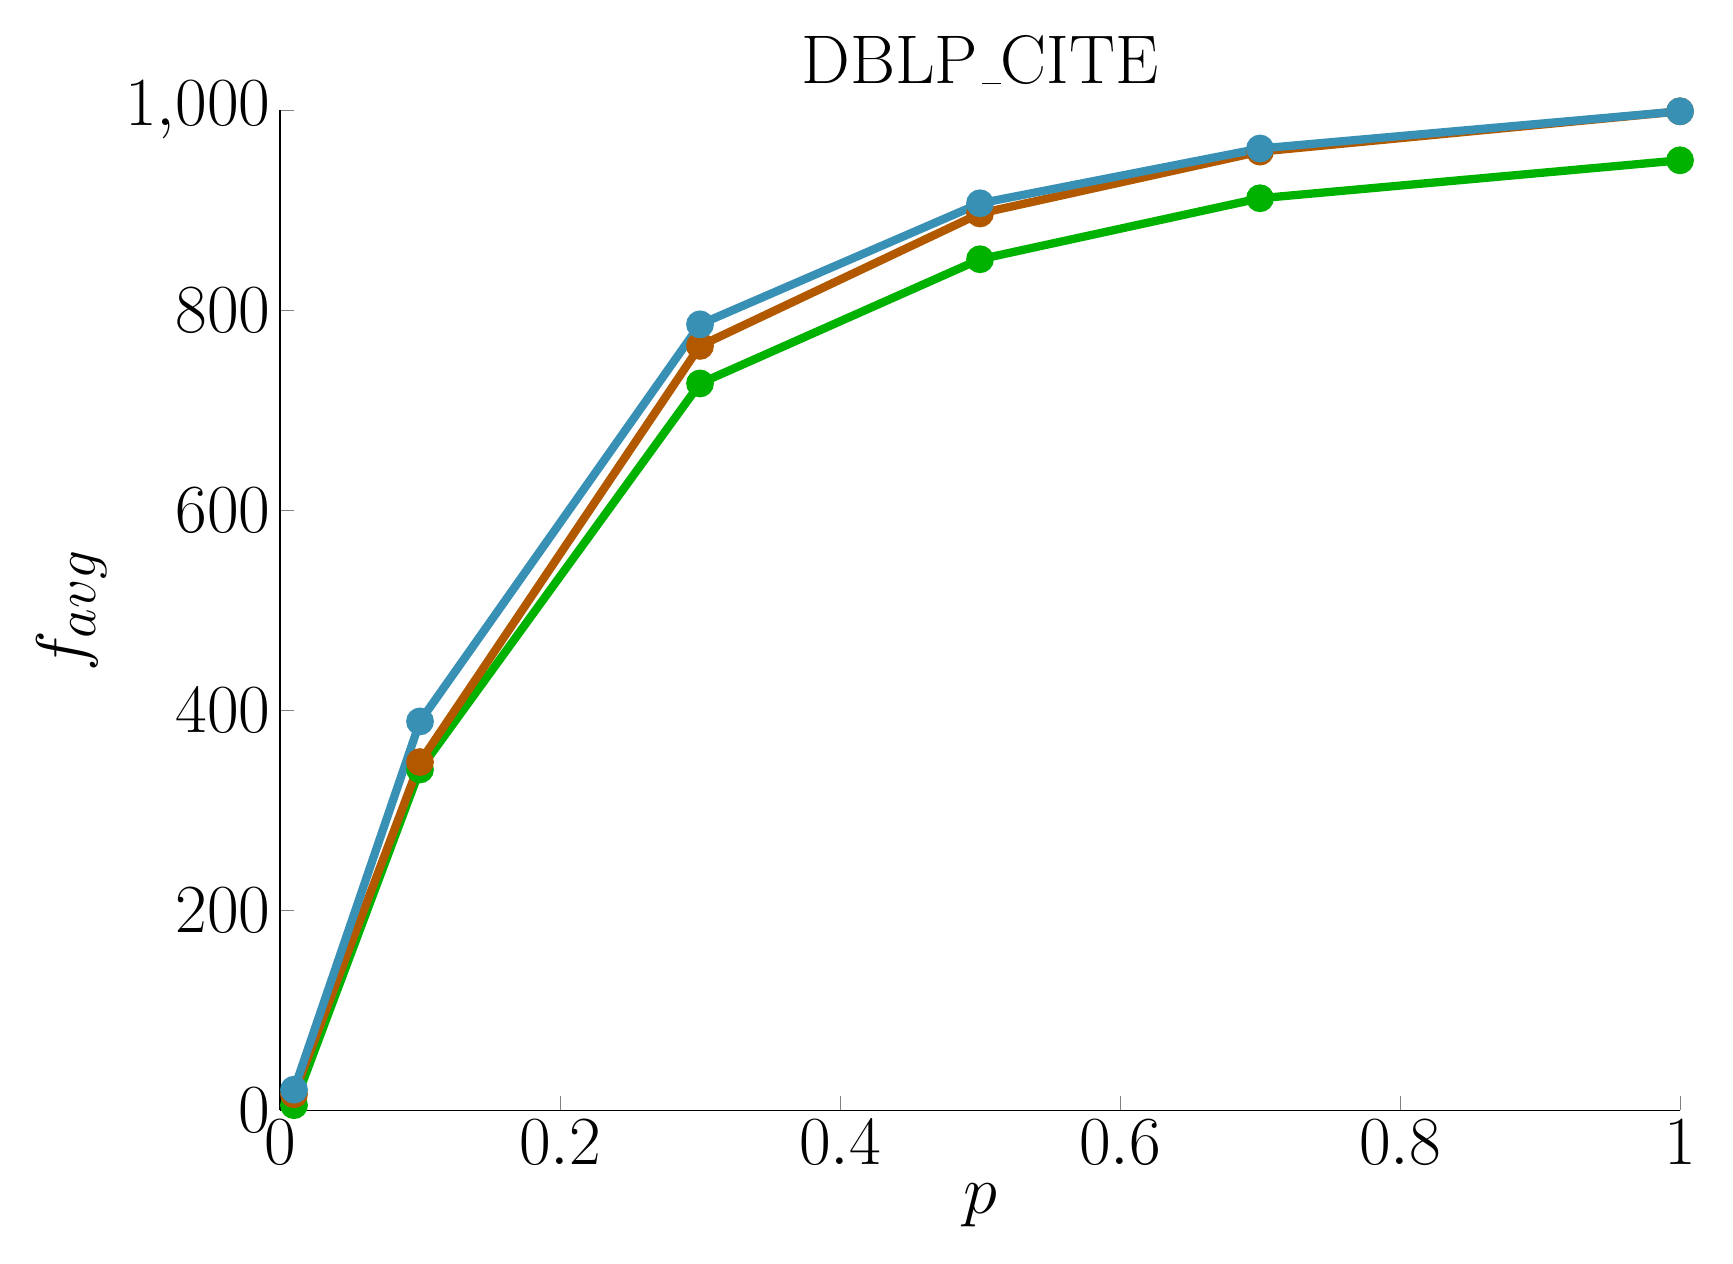
\begin{tikzpicture}

\begin{axis}[%
title style={font=\Huge},
title=DBLP\_CITE,
tick label style={font=\Huge},
label style={font=\Huge},
legend style={font=\Huge},
view={0}{90},
width=7in,
height=5in,
scale only axis,
xmin=0, xmax=1,
xtick={0, 0.2, 0.4, 0.6, 0.8, 1},
xlabel={$p$},
ymin=0, ymax=1000,
ytick={0, 200, 400, 600, 800, 1000},
ylabel={$f_{avg}$},
major tick length=5pt,
axis lines*=left,
legend cell align=left,
clip=false]

\addplot [
mark=*,
mark size=3.5pt,
color=green!70!black,
solid,
line width=3pt
]
coordinates{
(0.01,5.1)(0.1,340.85)(0.3,726.85)(0.5,851.05)(0.7,912.05)(1,950.0)
};

\addplot [
mark=*,
mark size=3.5pt,
color=orange!70!black,
solid,
line width=3pt
]
coordinates{
(0.01,16.0)(0.1,348.25)(0.3,764.4)(0.5,896.85)(0.7,958.7)(1,999.0)
};

\addplot [
mark=*,
mark size=3.5pt,
color=cyan!70!black,
solid,
line width=3pt
]
coordinates{
(0.01,20.65)(0.1,388.9)(0.3,785.95)(0.5,907.0)(0.7,961.8)(1,999.0)
};

\end{axis}
\end{tikzpicture}
\end{document}
